\section{openPOWERLINK Simulation}
\begin{frame}{openPOWERLINK Simulation}
    \begin{itemize}
        \item Separation of connection to openPOWERLINK stack from simulation modules.
        \item Reusability for different used stack configurations.
        \item Modularity for developing different Demo applications.
    \end{itemize}

    \begin{block}{Multiple Instances}
        \begin{itemize}
            \item Data and states stored in static variables
            \item Usage of openPOWERLINK library as shared library
            \item Multiple instances of shared library within memory
            \item Manual resolving and handling of different copies of shared library
        \end{itemize}
    \end{block}
\end{frame}

\begin{frame}{Simulation Hierarchy}
    \begin{columns}
        \begin{column}{0.43\textwidth}
            \begin{block}{Simulation interface}
                {\scriptsize
                     \begin{itemize}
                    \item Connection to stack
                    \item Handling of multiple stack instances
                    \item Static functions for function pointer
                \end{itemize}}
            \end{block}
            \begin{block}{Simulation modules}
                {\scriptsize
                \begin{itemize}
                    \item Representation of stack structure
                    \item Implementation of required functionalities
                \end{itemize}}
            \end{block}
        \end{column}
        \begin{column}{0.57\textwidth}
            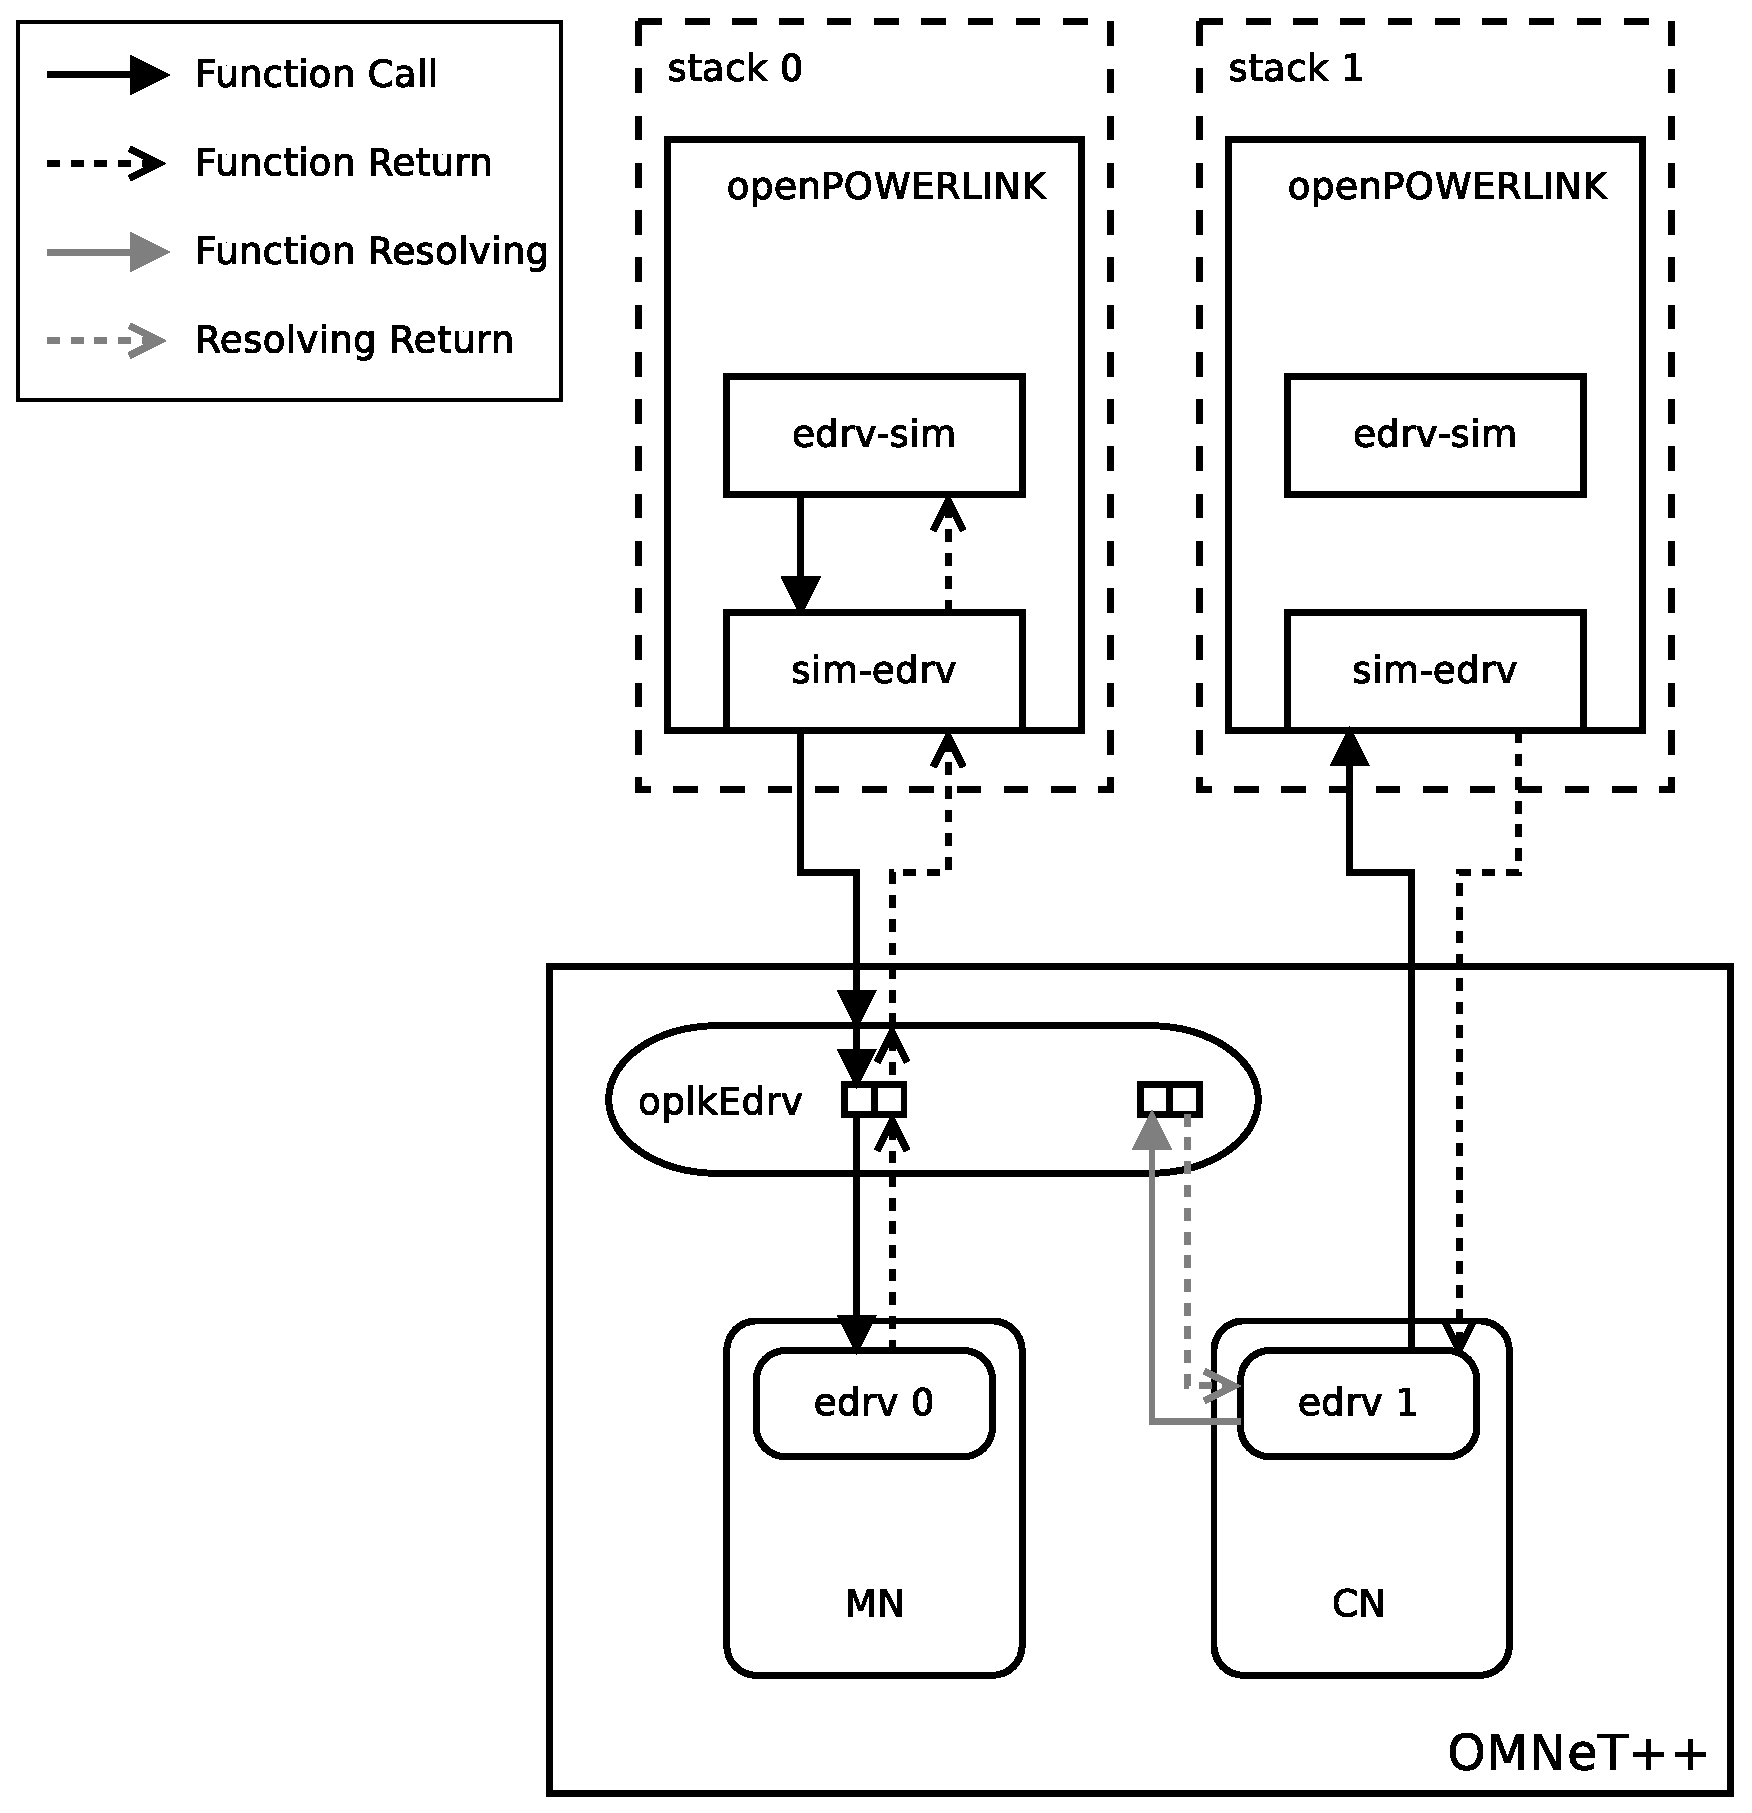
\includegraphics[height=0.85\textheight]{../../thesis/images/simulation_instances.eps}
        \end{column}
    \end{columns}
\end{frame}

\begin{frame}{Generic node, MN, CN}
    %TODO explain composition of compound stack module
    \begin{columns}
        \begin{column}{0.5\textwidth}
            \begin{block}{Stack module}
                \begin{itemize}
                    \item Structure of simulated openPOWERLINK stack
                    \item Basic functionalities for each node (MN, CN)
                    \item Message handling in between modules
                    \item Base classes for specific implementations
                \end{itemize}
            \end{block}
        \end{column}
        \begin{column}{0.5\textwidth}
                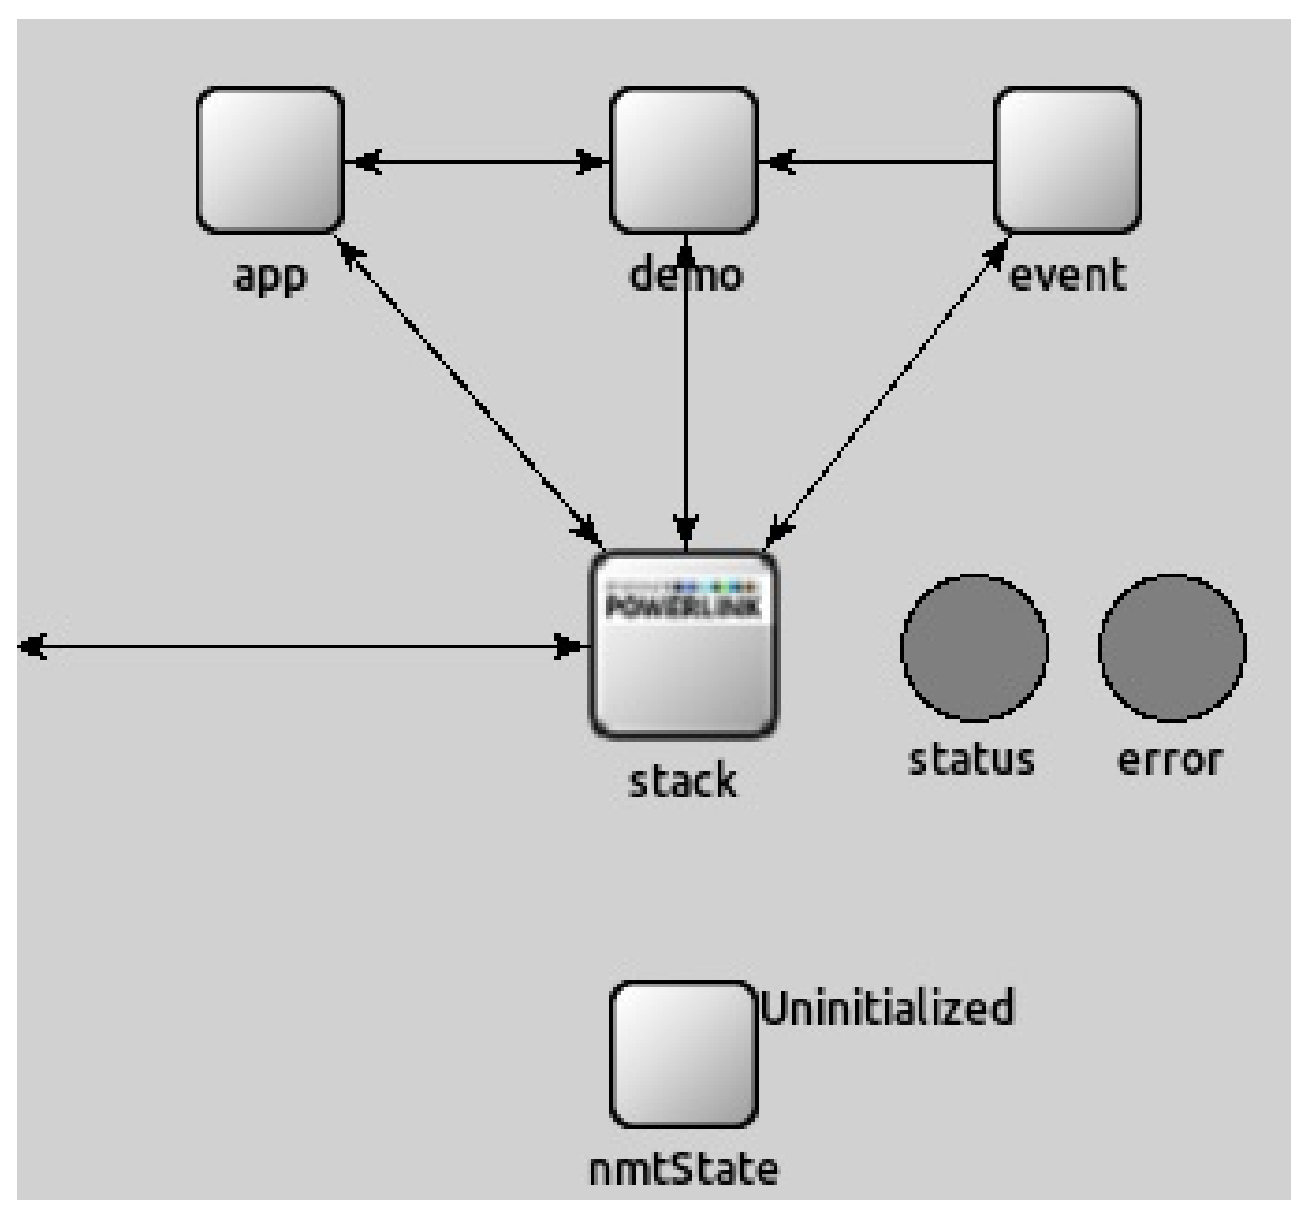
\includegraphics[width=0.9\textwidth]{../../thesis/images/simulation_genericnode.eps}
        \end{column}
    \end{columns}
\end{frame}

\begin{frame}{Further Development}
    \begin{block}{Enhancements}
        \begin{itemize}
            \item Usage of INET functionalities
            \item Implementation of different modularities
            \item Implementation of multiple demo networks/applications
        \end{itemize}
    \end{block}
    \begin{block}{Publication}
        \begin{itemize}
            \item Integration of the simulation stub within the openPOWERLINK stack 2.5.0
            \item Hosting on GitHub\\
            \url{https://github.com/OpenAutomationTechnologies/openPOWERLINK\_omnetpp}
        \end{itemize}
    \end{block}
\end{frame}